\section*{Введение}
\addcontentsline{toc}{section}{Введение}
Практически каждая команда разработчиков при создании программного продукта использует различные решения для контроля выполненных задач,
такими, как, например Gitlab issues или Redmine.
Без использования таких инструментов отслеживание вклада каждого человека в работу над продуктом становиться затруднительной задачей.

Исходя из важности использования таких решений, целью работы была поставлена задача разработки клиент-серверного программного обеспечения
с подобным функционалом, с добавлением в него элементов управления персоналом (работниками) и проектами (задачами),
используя собственный опыт разработки кроссплатформенного программного обеспечения с элементами интерфейса.


\clearpage
\section{Постановка задачи}
В процессе проектирования архитектуры приложения-клиента было решено реализовать следующий функционал:
\begin{enumerate}
    \item Авторизация работника, смена пароля работником;
    \item Добавление и увольнение работников;
    \item Создание и завершение проектов;
    \item Назначение проектов работнику;
    \item Редактирование данных работников и проектов;
    \item Отображение назначенных работнику проектов;
    \item Отображения списка работников, назначенных на конкретный проект.
\end{enumerate}

Серверная часть должна была выполнять запросы клиента, оперировать данными в БД, а также отвечать за аутентификацию пользователей в системе.
Исходя из этого серверная часть должна была иметь следующий функционал:
\begin{enumerate}
    \item Обработка запросов, поступающих от клиента;
    \item Поддержка защищенного соединения;
    \item Возможность одновременного ответа на несколько запросов;
    \item Поддержка кодов состояния HTTP;
    \item Контроль доступа к данным БД.
\end{enumerate}


\clearpage
\section{Используемые технологии}
Разработка клиент-серверных приложений влечет за собой необходимость в использовании множества технологий.
Необходим выбор протокола передачи данных, формата самих данных, способа их защиты, а также вида базы данных для их хранения.
Также неотъемлемой частью работы является выбор языка программирования для реализации задуманного функционала.

\begin{definition}
    <<Клиент --- сервер>> --- вычислительная или сетевая архитектура, в которой задания или сетевая нагрузка распределены между поставщиками услуг,
    называемыми серверами, и заказчиками услуг, называемыми клиентами. Фактически клиент и сервер --- это программное обеспечение.
    Обычно эти программы расположены на разных вычислительных машинах и взаимодействуют между собой через вычислительную сеть посредством сетевых протоколов.
\end{definition}

\begin{definition}
    Протокол передачи данных --- набор соглашений интерфейса логического уровня, которые определяют обмен данными между различными программами.
    Эти соглашения задают единообразный способ передачи сообщений и обработки ошибок.
\end{definition}

Для поддержки защищенного соединения между клиентом и сервером было принято решение использовать протокол HTTPS.
\begin{definition}
    HTTPS --- расширение протокола HTTP для поддержки шифрования в целях повышения безопасности.
    Данные в протоколе HTTPS передаются поверх криптографических протоколов SSL или TLS.
\end{definition}

\begin{definition}
    HTTP --- протокол прикладного уровня передачи данных изначально --- в виде гипертекстовых документов в формате <<HTML>>.
\end{definition}

Для упрощения процесса взаимодействия клиента и сервера был разработан собственный API,
с помощью которого происходит составление запросов и структурирование отправляемых данных.
\begin{definition}
    API --- описание способов (набор классов, процедур, функций, структур или констант),
    которыми одна компьютерная программа может взаимодействовать с другой программой.
\end{definition}

Данные между клиентом и сервером было решено передавать с помощью POST-запросов в формате JSON.
\begin{definition}
    POST --- один из многих методов запроса, поддерживаемых HTTP протоколом, используемым во Всемирной паутине.
    Метод запроса POST предназначен для запроса, при котором веб-сервер принимает данные, заключённые в тело сообщения, для хранения.
    Он часто используется для загрузки файла или представления заполненной веб-формы.
\end{definition}

\begin{definition}
    JSON --- текстовый формат обмена данными, основанный на JavaScript, как и многие другие текстовые форматы, он легко читается людьми.
\end{definition}

Для безопасной передачи данных аутентификации на сервер используется технология JSON Web Token (JWT).
\begin{definition}
    JSON Web Token (JWT) --- это открытый стандарт (RFC 7519) для создания токенов доступа, основанный на формате JSON.
    Как правило, используется для передачи данных для аутентификации в клиент-серверных приложениях.
\end{definition}

Исходя из личного опыта разработки, в качестве основного языка программирования был выбран Python версии 3.7.
\begin{definition}
    Python --- высокоуровневый язык программирования общего назначения, ориентированный на повышение производительности разработчика и читаемости кода.
    Синтаксис ядра Python минималистичен. В то же время стандартная библиотека включает большой объём полезных функций.
    Python поддерживает структурное, объектно-ориентированное, функциональное, императивное и аспектно-ориентированное программирование.
    Основные архитектурные черты --- динамическая типизация, автоматическое управление памятью, полная интроспекция, механизм обработки исключений,
    поддержка многопоточных вычислений, высокоуровневые структуры данных. Поддерживается разбиение программ на модули, которые, в свою очередь,
    могут объединяться в пакеты.
\end{definition}

Для создания интерфейса клиента было решено использовать PyQt5 в связке с конструктором интерфейса Qt designer.
Такой выбор обусловлен кроссплатформенностью этого инструмента, большой базой компонентов и возможностью создания собственных,
а также подробной документацией Qt5.
\begin{definition}
    Qt  --- кроссплатформенный фреймворк для разработки программного обеспечения на языке программирования C++.
    Включает в себя все основные классы, которые могут потребоваться при разработке прикладного программного обеспечения,
    начиная от элементов графического интерфейса и заканчивая классами для работы с сетью, базами данных и XML.
    Является полностью объектно-ориентированным, расширяемым и поддерживающим технику компонентного программирования.
\end{definition}

\begin{definition}
    PyQt --- набор <<привязок>> графического фреймворка Qt для языка программирования Python, выполненный в виде расширения Python.
\end{definition}

\begin{definition}
    Qt Designer --- кроссплатформенная свободная среда для разработки графических интерфейсов (GUI) программ, использующих библиотеку Qt.
\end{definition}

Для хранения и обработки данных использован виртуальный сервер (VPS) со следующим окружением:
\begin{enumerate}
    \item Сервер базы данных MongoDB;
    \item Nginx для работы API;
    \item Gunicorn в качестве WSGI сервера;
    \item Серверная часть существует в виде Docker контейнера.
\end{enumerate}

При выборе системы управления базами данных выбор пал на MongoDB. Этот выбор обусловлен открытым исходным кодом продукта,
а также желанием получить опыт использования NoSQL СУБД в проекте.
\begin{definition}
    MongoDB --- документоориентированная система управления базами данных (СУБД) с открытым исходным кодом,
    не требующая описания схемы таблиц. Классифицирована как NoSQL, использует JSON-подобные документы и схему базы данных.
\end{definition}

В качестве веб сервера был выбран Nginx. Для взаимодействия веб-сервера и кода на языке программирования Python был использован WSGI-сервер Gunicorn.
\begin{definition}
    Nginx --- веб-сервер и почтовый прокси-сервер, работающий на UNIX-подобных операционных системах.
\end{definition}

\begin{definition}
    Gunicorn (Green Unicorn) --- WSGI HTTP сервер, написанный на языке программирование Python, для UNIX систем.
\end{definition}

\begin{definition}
    UNIX --- семейство переносимых, многозадачных и многопользовательских операционных систем, которые основаны на идеях оригинального проекта AT\&T Unix,
    разработанного в 1970-х годах в исследовательском центре Bell Labs. Операционные системы семейства Unix характеризуются модульным дизайном,
    в котором каждая задача выполняется отдельной утилитой, взаимодействие осуществляется через единую файловую систему,
    а для работы с утилитами используется командная оболочка.
\end{definition}

\begin{definition}
    WSGI --- стандарт взаимодействия между Python-программой, выполняющейся на стороне сервера, и самим веб-сервером.
\end{definition}

Почти все компоненты, необходимые для работы сервера, были развернуты с помощью технологии Docker.
\begin{definition}
    Docker --- программное обеспечение для автоматизации развёртывания и управления приложениями в средах с поддержкой контейнеризации.
    Позволяет <<упаковать>> приложение со всем его окружением и зависимостями в контейнер, который может быть перенесён на любую Linux-систему.
\end{definition}


\clearpage
\section{Этапы создания сервера}
\subsection{Создание и настройка сервера}
Для разработки и отладки клиент-серверной архитектуры можно было обойтись созданием и настройкой домашнего локального сервера.
Но, для доступности из любого места и для реального видения скорости обработки данных, был арендован VPS сервер на территории России.

\begin{definition}
    VPS --- услуга предоставления в аренду так называемого виртуального выделенного сервера.
    В плане управления операционной системой по большей части она соответствует физическому выделенному серверу.
    В частности: root-доступ, собственные IP-адреса, порты, правила фильтрования и таблицы маршрутизации.
\end{definition}

В качестве операционной системы VPS сервера была выбрана Linux Ubuntu 18.04 LTS с базовой настройкой доступа и безопасности.
\begin{definition}
    Ubuntu --- операционная система, основанная на Debian GNU/Linux. Основным разработчиком и спонсором является компания Canonical. 
    В настоящее время проект активно развивается и поддерживается свободным сообществом.
\end{definition}

После этого необходимо установить Docker, который позволит начать развертку Docker-контейнера с собранным комплектом для работы MongoDB,
Gunicorn и логики архитектуры. Так же необходим Docker-контейнер с настроенным Nginx.
Все эти инструменты возможно установить и использовать без использования Docker,
но тогда будет утерена мобильность архитектуры, которая может понадобится в случае смены VPS сервера на другой.


\clearpage
\subsection{Настройка работы HTTPS}
Для безопасной передачи данных между клиентом и сервером была реализована
поддержка протокола передачи данных HTTPS. Для этого на сервере был получен цифровой SSL сертификат.
\begin{definition}
    Цифровой сертификат --- выпущенный удостоверяющим центром электронный или печатный документ,
    подтверждающий принадлежность владельцу открытого ключа или каких-либо атрибутов.
    Сертификат открытого ключа удостоверяет принадлежность открытого ключа некоторому субъекту, например, пользователю.
    Сертификат открытого ключа содержит имя субъекта, открытый ключ, имя удостоверяющего центра,
    политику использования соответствующего удостоверяемому открытому ключу закрытого ключа и другие параметры, заверенные подписью удостоверяющего центра.
\end{definition}

В данном случае, для шифрования трафика можно было обойтись созданием самозаверенного сертификата.
\begin{definition}
    Самозаверенный сертификат --- специальный тип сертификата, подписанный самим его субъектом. Технически данный тип ничем не отличается от сертификата,
    заверенного подписью удостоверяющего центра, только вместо передачи на подпись в удостоверяющий центр пользователь создаёт свою собственную сигнатуру.
    Создатель сертификата сам является в данном случае удостоверяющим центром.
\end{definition}

Но, вместо создания самозаверенного сертификата было решено обратится к центру сертификации Let’s Encrypt,
что позволило достичь высоких стандартов безопасности (рис. \ref{fig:https_score}).
\begin{definition}
    Let’s Encrypt --- центр сертификации, предоставляющий бесплатные криптографические сертификаты X.509 для TLS-шифрования (HTTPS).
    Процесс выдачи сертификатов полностью автоматизирован. Проект создан для того,
    чтобы большая часть интернет-сайтов смогла перейти к шифрованным подключениям (HTTPS). В отличие от коммерческих центров сертификации,
    в данном проекте не требуется оплата, переконфигурация веб-серверов, использование электронной почты,
    обработка просроченных сертификатов, что делает процесс установки и настройки TLS-шифрования значительно более простым.
\end{definition}

\begin{figure}[h]
    \centering
    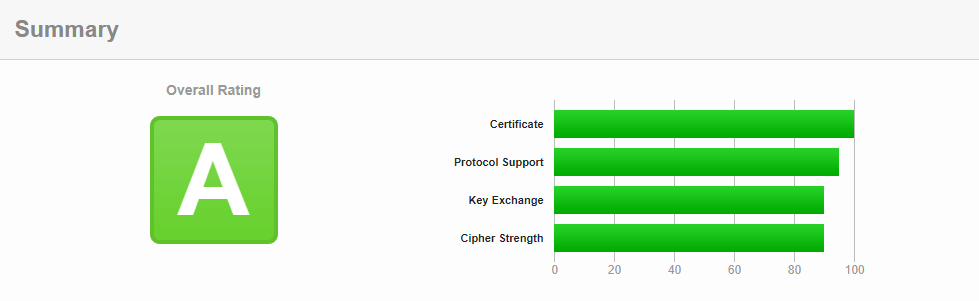
\includegraphics[width=1\linewidth]{img/https_score.png}
    \caption{Рейтинга безопасности для SSL-сертификата сервера.}
    \label{fig:https_score}
\end{figure}


\clearpage
\subsection{Интеграция технологии JSON Web Token (JWT)}
Аутентификация пользователя на сервере происходит с помощью логина и пароля, после чего клиенту выдается токен для дальнейшего отправления данных.
По истечению некоторого времени, этот токен необходимо обновить по средствам повторной аутентификации.
Для структурирования и шифрования данного токена ьыла использована технология JWT.

Токен представляет собой набор данных из трех секций в зашифрованном виде (рис. \ref{fig:token1}).
\begin{figure}[h]
    \centering
    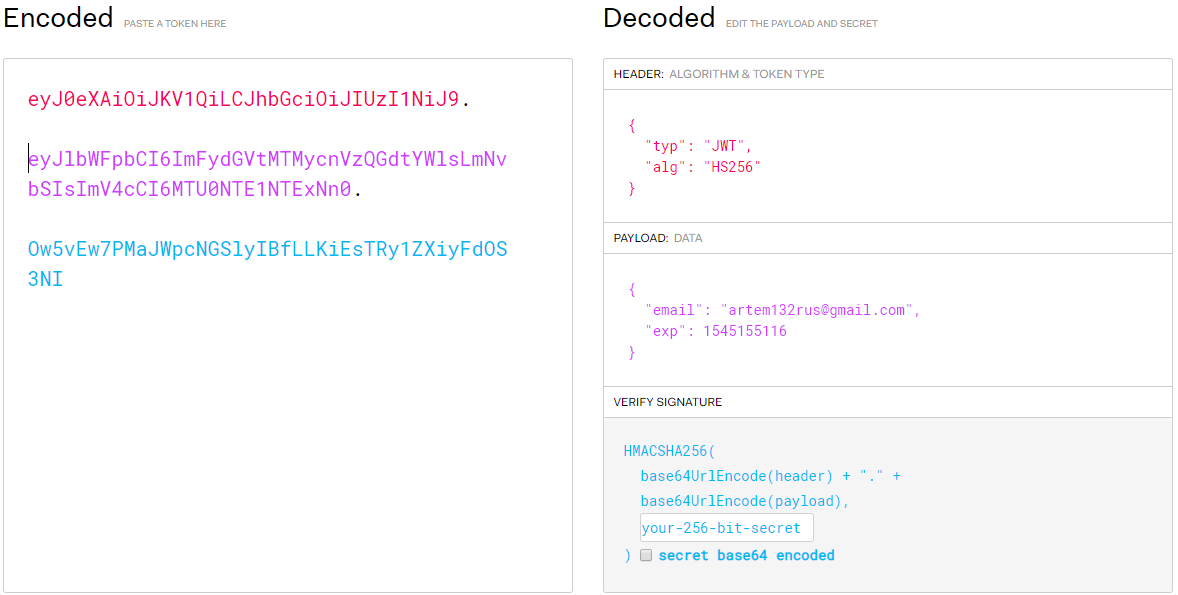
\includegraphics[width=1\linewidth]{img/token1.png}
    \caption{Cтруктура токена.}
    \label{fig:token1}
\end{figure}
Первая секция (HEADER) отвечает за информацию об используемых технологиях (JWT) и шифровании (HS256).
Во второй секции (PAYLOAD) записан владелец токена (email), а также время, когда этот токен выдан.
Третья секция (VERIFY SIGNATURE) содержит хеш-суммы первой и второй секции, для проверки токена на подлинность.
Для безопасности, третья секция токена шифруется перед отправкой. Весь токен отправляется в кодировке Base64.
\begin{definition}
   Base64 --- стандарт кодирования двоичных данных при помощи только 64 символов ASCII.
\end{definition}


\clearpage
\subsection{Разработка собственного API}
Для взаимодействия сервера и клиента было разработано собственноое API, которое удовлетворяет всем нуждам проекта.
Созданное API позволяет передавать данные по средствам POST-запроса в формате JSON (рис. \ref{fig:req}).
Для оптимизации передачи данных, была добавлена возможность объединять множественные запросы в один POST-запрос перед отправкой.
Ответ от сервера так же приходит в формате JSON (рис. \ref{fig:ans}), а если запрос был множественным,
ответ на него будет содержать вложенные данные для ответа на каждый запрос.
\begin{figure}[h]
    \centering
    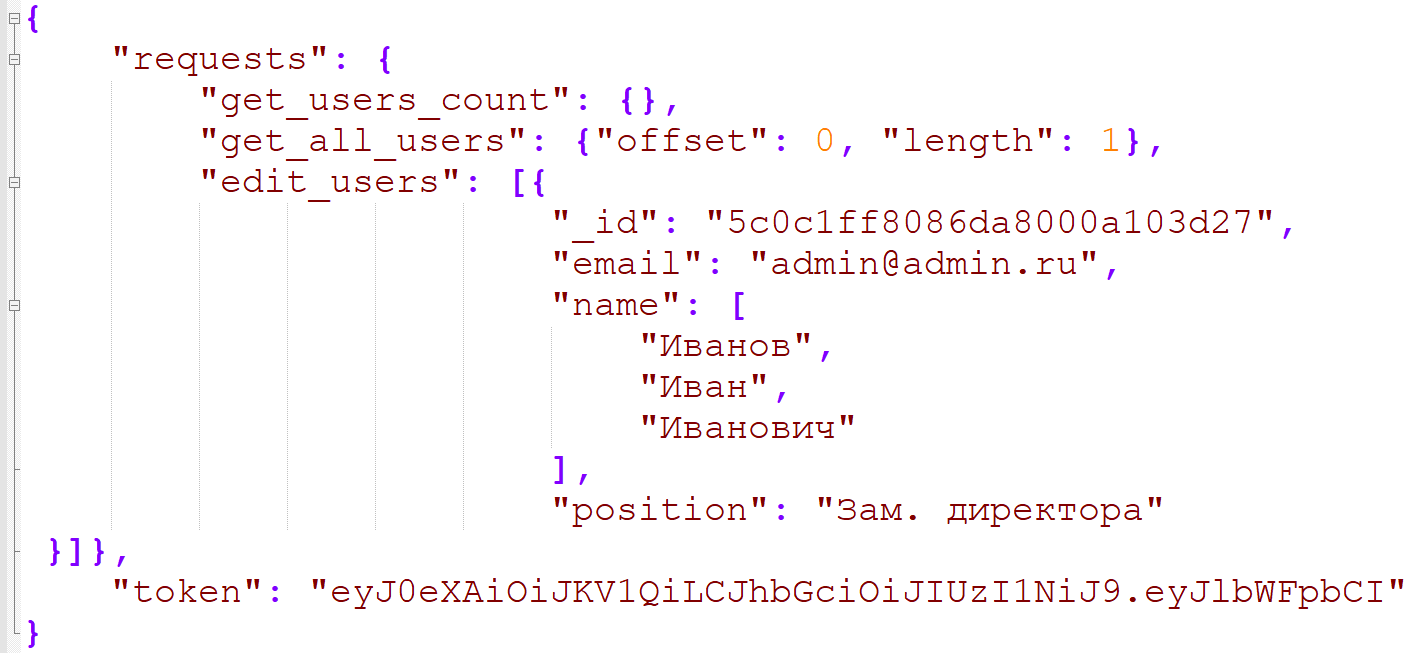
\includegraphics[width=1\linewidth]{img/req.png}
    \caption{Формат запроса к API. В данном случае, выполняется запрос на получение количества пользователей,
    получения данных одного из них, а также последующие редактирование этого пользователя.}
    \label{fig:req}
\end{figure}

\begin{figure}[h]
    \centering
    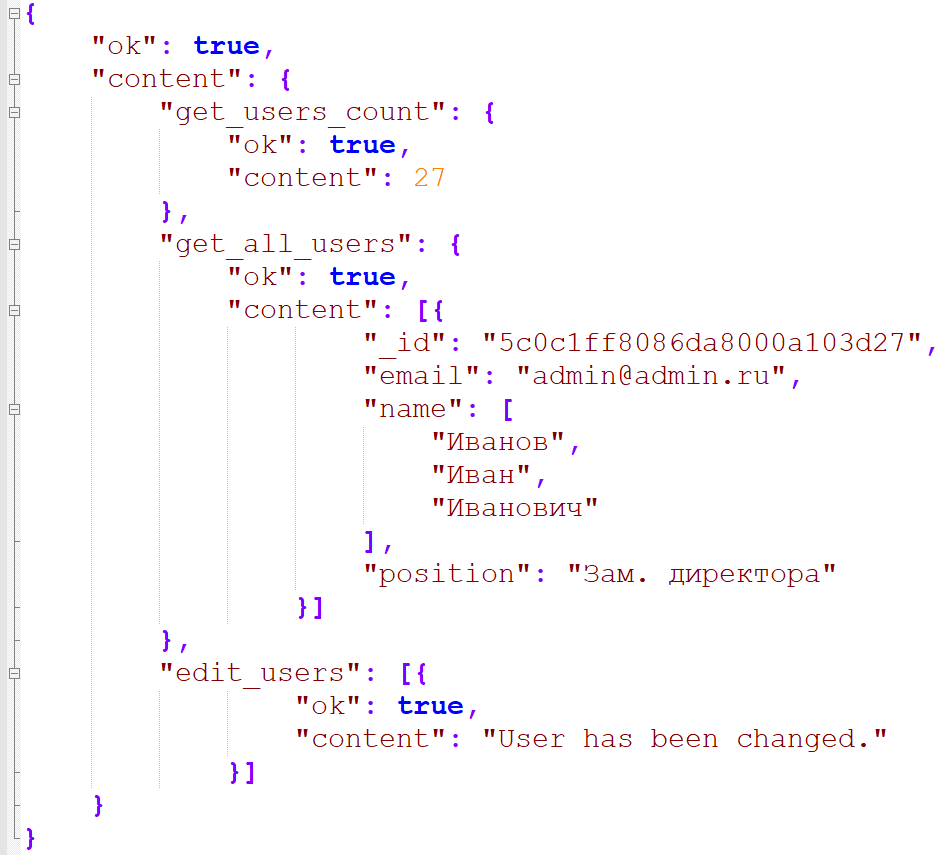
\includegraphics[width=1\linewidth]{img/ans.png}
    \caption{Ответ сервера на запрос, представленный на рис. \ref{fig:req}. Данные для каждого запроса были объединены в один JSON файл.}
    \label{fig:ans}
\end{figure}


\clearpage
\subsection{Реализация серверной части}
Основная логика работы с БД и обработки запросов реализована за счет возможностей языка программирования Python.
Для обращения к СУБД MongoDB (чтение, запись) используется библиотека pymongo. Для интеграции технологии JSON Web Token (JWT) используется библиотека jwt.
Для обработки json файлов используется библиотека json.

Каждое логическое действие представляет собой обособленную функцию, которая будет вызвана при необходимости.

\lstinputlisting[caption={Функция сервера для создания токена для клиента, прошедшего аутентификацию.}, language=Python, breaklines]{code/create_token_server_func.py}

\lstinputlisting[caption={Функция сервера для проверки токена клиента.}, language=Python, breaklines]{code/check_token_server_func.py}

\lstinputlisting[caption={Функция сервера для авторизации клиента.}, language=Python, breaklines]{code/auth_server_func.py}

При взаимодействии с сервером используются коды состояния HTTP для сообщения о статусе различных операций.
\begin{definition}
    Код состояния HTTP --- часть первой строки ответа сервера при запросах по протоколу HTTP (HTTPS).
    Он представляет собой целое число из трёх десятичных цифр. Первая цифра указывает на класс состояния.
    За кодом ответа обычно следует отделённая пробелом поясняющая фраза на английском языке, которая разъясняет человеку причину именно такого ответа.
\end{definition}

Примерами таких кодов могут быть:
\begin{itemize}
    \item 200 OK (<<хорошо>>);
    \item 400 Bad Request (<<плохой или неверный запрос>>);
    \item 404 Not Found (<<не найдено>>).
\end{itemize}

\lstinputlisting[caption={
    Функция сервера для связывания проекта с работником. В ней присудствует множество условий проверки, каждый из которых даст некий код состояния HTTP.
    },language=Python, breaklines]{code/assign_to_projects_server_func.py}

Для проверки правильной работы всех модулей сервера были использованы unit-тесты, исходные коды которых содержатся в файле tests.py.
\begin{definition}
    Юнит-тестирование --- процесс в программировании, позволяющий проверить на корректность отдельные модули исходного кода программы,
    наборы из одного или более программных модулей вместе с соответствующими управляющими данными, процедурами использования и обработки. 
\end{definition}
\lstinputlisting[caption={Функция сервера для тестирования удаления пользователя из базы данных.}, language=Python, breaklines]{code/test_del_users_server_func.py}


\clearpage
\section{Этапы создания клиента}
\subsection{Настройка системы для разработки клиента}
Разработка клиентской части происходила в ОС Windows 10, где и решено было установить необходимые инструменты.

Для установки языка программирования Python с официального сайта был взят установочный файл и запущен с правами администратора.
Дальнейшая настройка не требовалась.

Установка PyQt5 возможна с помощью менеджера пакетов pip, который идет в комплекте с языком программирования Python.
После этого настройка не требуется. Такие вспомогательные инструменты, как Qt Designer будут установлены автоматически.
\begin{definition}
    pip --- система управления пакетами, которая используется для установки и управления программными пакетами, написанными на языке программирования Python.
\end{definition}


\clearpage
\subsection{Создание интерфейса}
Для создания макета интерфейса клиента использовался инструмент Qt Designer (рис. \ref{fig:qtdesigner}),
позволяющий сразу увидеть результаты работы, включив превью-режим. Qt Designer создает UI-файлы, которые возможно конвертировать в необходимый формат.
В данном случае, конвертирование происходило в формат языка программирования Python.
\begin{figure}[h]
    \centering
    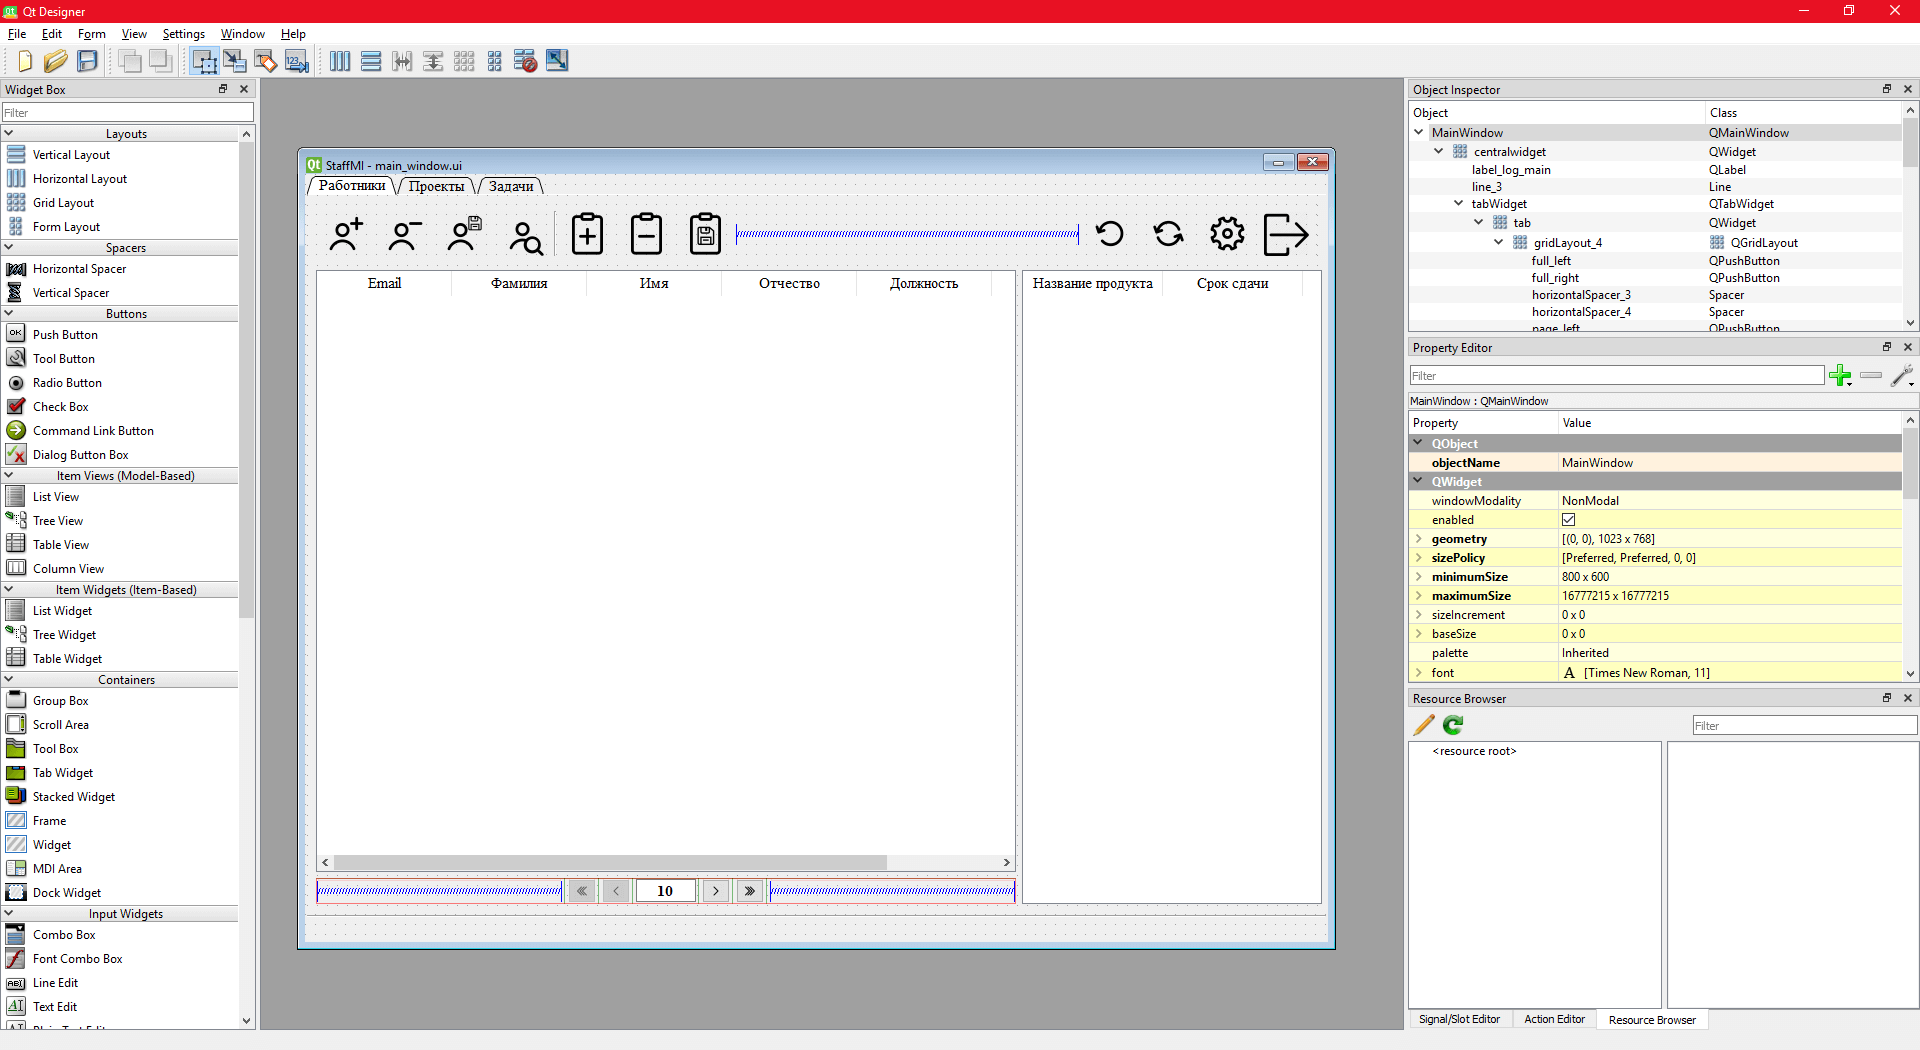
\includegraphics[width=1\linewidth]{img/qtdesigner.png}
    \caption{Редактирование главного меню клиента в Qt Designer.}
    \label{fig:qtdesigner}
\end{figure}

Для просмотра результатов работы с интерфейсом в данном инструменте присудствует превью-режим.
Для проверки всех интерактивных элементов интерфейса конвертированный UI-файл был подключен к программе с минимальным echo-функционалом.


\clearpage
\subsection{Реализация клиентской части}
Основная логика работы и обработки событий в интерфейсе клиента реализована за счет языка программирования Python.
Для обращения серверу используется собственное API. Для обработки json файлов используется библиотека json.
Для работы с Qt5 используется библиотека PyQt5 и ее компоненты (QtWidgets, QtCore, QtGui и т.д.).
Для работы с post-запросами используется библиотека requests.

В файле db\_api.py реализована работа собственного API. Он представляет список функций-запросов к серверу, которые вызываются по мере необходимости.

\lstinputlisting[caption={Функция клиента для авторизации пользователя на сервере.}, language=Python, breaklines]{code/auth_client_func.py}

\lstinputlisting[caption={Функция клиента для отправки запроса на сервер и последующей обработки ответа.}, language=Python, breaklines]{code/send_query_client_func.py}

В файле main\_logic.py реализована вся логика работы интерфейса.
Различные нажатия, события и процессы обрабатывается с помощью методов того класса, к которому они относятся.
Разделение по классам была необходима для реализации принципа многооконного интерфейса.
Каждый такой класс имеет свои методы для обработки различных действий и событий. В данный момент таких классов 5, а именно:
\begin{itemize}
    \item miWindow --- класс, отвечающий за главное окно интерфейса.
    \item loginStackWindow --- класс, отвечающий за окно авторизации и смены пароля пользователя.
    \item inprojectDialogWindow --- класс, отвечающий за диалог добавления работника в проект.
    \item newProjectDialogWindow --- класс, отвечающий за диалог создания нового проекта.
    \item newUserDialogWindow --- класс, отвечающий за диалог добавления нового пользователя.
\end{itemize}

Главенствующим классом считается miWindow, он же и самый объемный. Несмотря на это, первым делом, пользователь увидит окно авторизации, 
за которое отвечает класс loginStackWindow, в котором и будет создан объект главного класса.


\clearpage
\subsection{Логика работы клиента}
После запуска приложения, пользователь увидит окно авторизации (рис. \ref{fig:auth_window_win}).
В нем же он может изменить пароль от своей учетной записи. После успешного прохождения этапа аутентификации,
пользователь попадает на главное окно интерфейса (рис. \ref{fig:main_window_win}), где доступны подменю работы с работниками и проектами.
Если же аутентификации не была успешной, будет выдана соотвтствующая ошибка (рис. \ref{fig:auth_login_error}), также как и в случае, если с сервером не была установлена связь.
\begin{figure}[h]
    \centering
    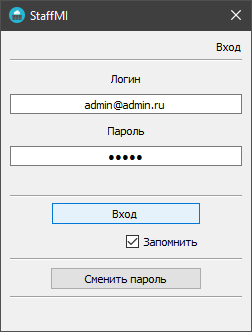
\includegraphics[width=0.4\linewidth]{img/auth_window_win.png}
    \caption{Окно авторизации пользователя.}
    \label{fig:auth_window_win}
\end{figure}
\begin{figure}[h]
    \centering
    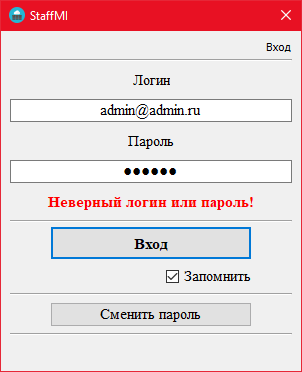
\includegraphics[width=0.4\linewidth]{img/login_error.png}
    \caption{Ошибка авторизации пользователя.}
    \label{fig:auth_login_error}
\end{figure}

В главном окне пользователь может отредактировать данные любого проекта или работника,
добавить новых (рис. \ref{fig:add_user_window_win}) (рис. \ref{fig:add_project_window_win}), связать выбранных работников с проектом,
а также удалять любые проекты и любых работников. Все изменения данных будут отображены специальными цветами:
\begin{itemize}
    \item Зеленый --- добавленная запись;
    \item Желтый --- отредактированная запись;
    \item Красный --- удаленная запись.
\end{itemize}

\begin{figure}[h]
    \centering
    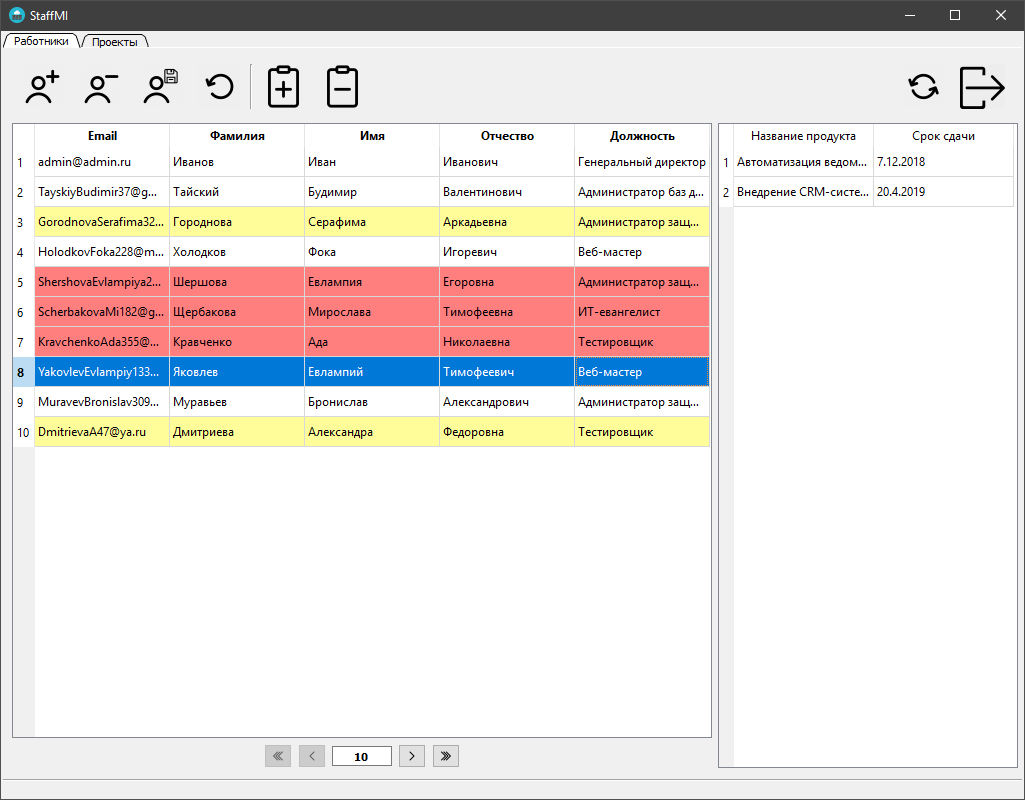
\includegraphics[width=1\linewidth]{img/main_window_win.png}
    \caption{Главное окно интерфейса.}
    \label{fig:main_window_win}
\end{figure}

\begin{figure}[h]
    \centering
    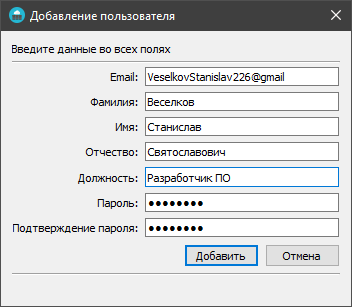
\includegraphics[width=0.5\linewidth]{img/add_user_window_win.png}
    \caption{Диалог добавления нового пользователя.}
    \label{fig:add_user_window_win}
\end{figure}

\begin{figure}[h]
    \centering
    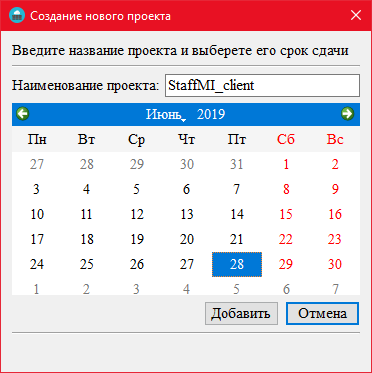
\includegraphics[width=0.5\linewidth]{img/add_project.png}
    \caption{Диалог добавления нового проекта.}
    \label{fig:add_project_window_win}
\end{figure}

Все данные, которые были изменены пользователем, будут хранится во временной памяти до тех пор, пока не будет дана команда отправки изменений на сервер.
Сделанные изменения можно отменить, если они еще не были отправлены на сервер.
Для предотвращения переизбытка используемой оперативной памяти используется постраничное отображение информации, размер этих страниц можно настроить.

В режиме реального времени происходит проверка соединения с сервером. Если произойдет разрыв соединения, пользователь будет предупрежден,
а часть функционала интерфейса станет недоступной для взаимодействия.

Для общения с сервером, клиенту необходимо передавать ему вместе с запросами актуальный токен.
Если был отправлен истекший токен, сервер отправит в ответе информацию об этом.
В этом случае, обновление истекшего токена происходит во время работы программы так,
что бы пользователь не замечал этого --- повторный ввод логина и пароля требоваться не будет.

За счет кроссплатформенности PyQt5, интерфейс клиента на других ОС не будет отличатся от интерфейса на ОС Windows 10 (рис. \ref{fig:main_window_linux}),
за исключением элементов интерфейса самой системы (например, стиль верхней панели окна).
\begin{figure}[h]
    \centering
    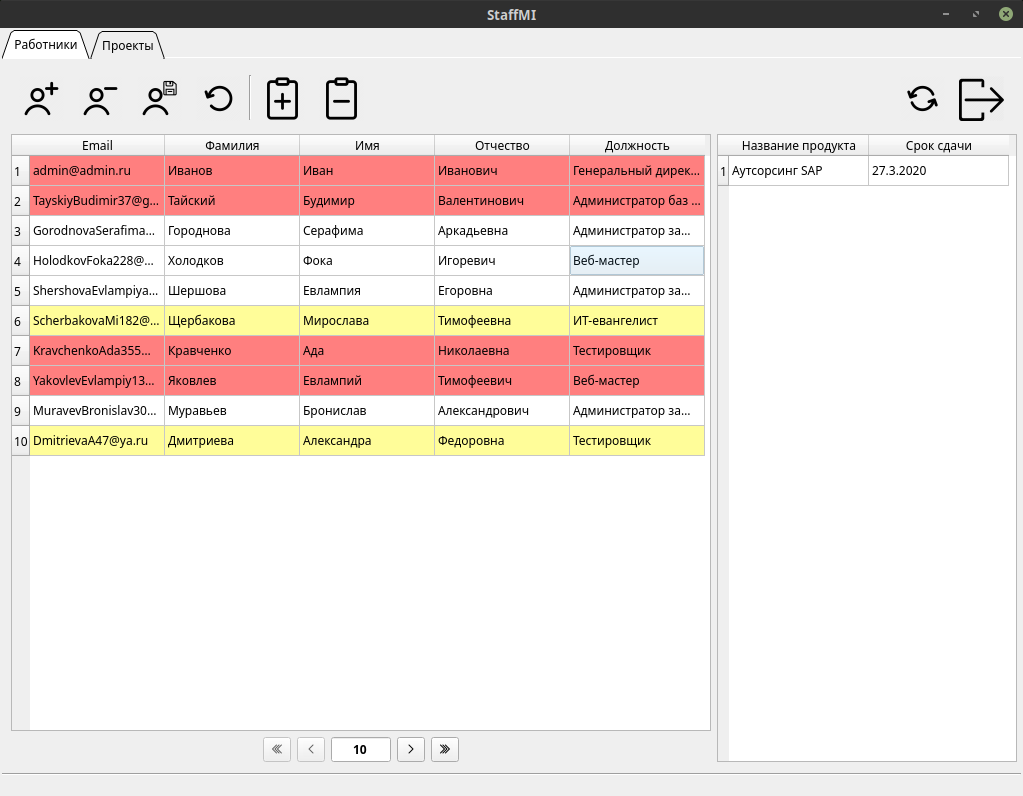
\includegraphics[width=1\linewidth]{img/main_window_linux.png}
    \caption{Главное окно интерфейса в ОС Linux Mint.}
    \label{fig:main_window_linux}
\end{figure}

\begin{figure}[h]
    \centering
    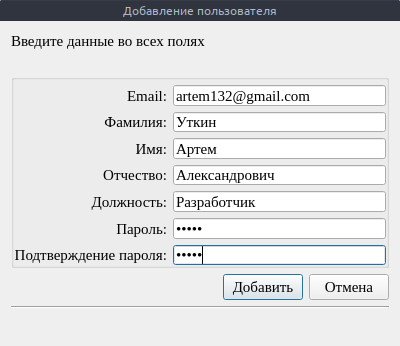
\includegraphics[width=0.5\linewidth]{img/add_user_linux.png}
    \caption{Диалог добавления нового пользователя в ОС Linux Mint.}
    \label{fig:add_user_linux}
\end{figure}

\begin{figure}[h]
    \centering
    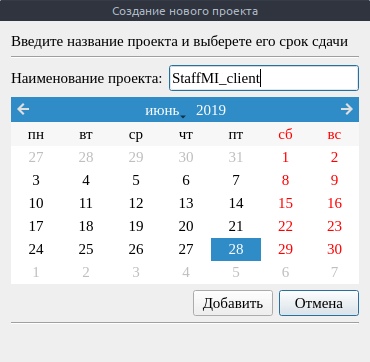
\includegraphics[width=0.5\linewidth]{img/add_project_linux.png}
    \caption{Диалог добавления нового проекта в ОС Linux Mint.}
    \label{fig:add_project_linux}
\end{figure}


\clearpage
\section{Заключение}
Современные технологии программирования предоставляют разработчикам неограниченные возможности для реализации своих идей.
В данной дипломной работе, с помощью перечисленных выше технологий и собственненного опыта разработки кроссплатформенного программного обеспечения
с элементами интерфейса было, разработано клиент-серверное приложение для управления персоналом (работниками) и проектами (задачами)
Создание данного ПО дало огромный толчок в понимании клиент-серверных архитектур, опыт работы с PyQt5,
а также позволило получить практический опыт разработки подобных решений.


\clearpage
\section{Приложение}
\subsection{Исходный код server/app.py}
\lstinputlisting[language=Python, breaklines]{code/app.py}


\clearpage
\subsection{Исходный код server/db.py}
\lstinputlisting[language=Python, breaklines]{code/db.py}


% \clearpage
% \subsection{Исходный код server/tests.py}
% \lstinputlisting[language=Python, breaklines]{code/tests.py}


\clearpage
\subsection{Исходный код client/db\_api.py}
\lstinputlisting[language=Python, breaklines]{code/db_api.py}


\clearpage
\subsection{Исходный код client/main\_logic.py}
\lstinputlisting[language=Python, breaklines]{code/main_logic.py}


\clearpage
\addcontentsline{toc}{section}{Список литературы}
\nocite{*}
\printbibliography{}
